\begin{problem}{1}
\textbf{Visualization}

As usual, in figure~\ref{double} we plotted the real space and the phase space
of the double pendulum, overlaying the two segments into the same plot. In addition,
we animated the double pendulum using the real space as shown in figure \ref{anim}.

Other interesting plots include figure ?, which compares the total energy over
time of the symplectic solution to a python built-in solution; figure
\ref{lyapunov} shows how the Lyapunov exponent varies with different initial
positions, as explained below. Finally, in figure ? we plotted the first
combinations of $\theta_{01}$ and $\theta_{02}$ that ``flip'' the pendulum, i.e.
either $\theta_1$ or $\theta_2$ goes above $\pi$.

\begin{figure}[ht!]
	\centering
	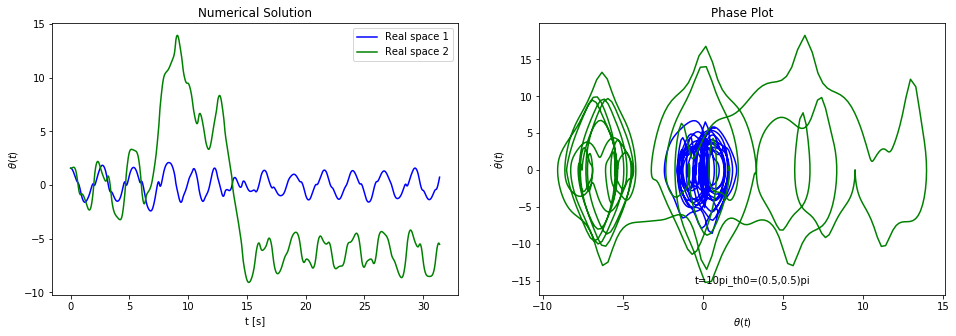
\includegraphics[scale=0.6]{../figures/t=10pi_th0=(05,05)pidoublePend.png}
	\caption{Trajectory of double pendulum}
	\label{double}
\end{figure}

\begin{figure}[ht!]
	\centering
	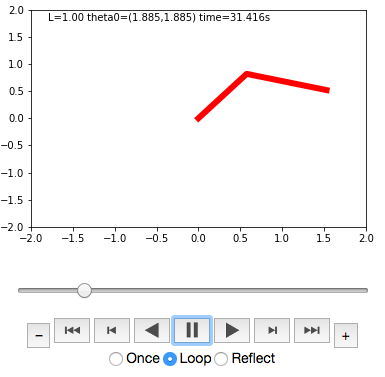
\includegraphics[scale=0.5]{../figures/doublePendAnim.png}
	\caption{Screenshot of double pendulum animation}
	\label{anim}
\end{figure}

\end{problem}

\begin{problem}{2}
\textbf{Lyapunov Exponent}

The Lyapunov exponent is a measure of the chaos in a system.  

\begin{figure}[ht!]
	\centering
	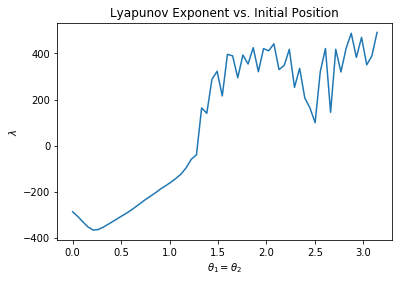
\includegraphics[scale=0.6]{../figures/lyapunov.png}
	\caption{}
	\label{lyapunov}
\end{figure}

\end{problem}

\begin{problem}{3}
\textbf{Transition to Chaos}

\begin{figure}[ht!]
	\centering
	%\includegraphics[scale=0.6]{../figures/.png}
	\caption{}
	\label{}
\end{figure}

\end{problem}

\begin{problem}{4}
\textbf{Time for First Flip}

\begin{figure}[ht!]
	\centering
	%\includegraphics[scale=0.6]{../figures/.png}
	\caption{}
	\label{}
\end{figure}

\end{problem}
